\section{Результаты моделирования}

\subsection{Параметры модели}

Расчёт выполняется для радиального подшипника скольжения с геометрией~\varGeomLetter{} и \varDimpleTypeGenitive{} микрорельефом. Сводные исходные данные представлены в таблице~\ref{tab:input_data}.

\begin{table}[H]
\small
\caption{Исходные данные для расчёта}
\label{tab:input_data}
\begin{tabularx}{\textwidth}{|X|c|c|}
\hline
\centering\textbf{Параметр} & \textbf{Значение} & \textbf{Размерность} \\
\hline
Радиус вала $R$ & \varRmm & мм \\
\hline
Радиальный зазор $c$ & \varCmkm & мкм \\
\hline
Длина подшипника $L$ & \varLmm & мм \\
\hline
Относительная длина $L/D$ & \varLD & -- \\
\hline
Полуось по оси $Z$, $a$ & \varDimpleAmm & мм \\
\hline
Полуось по оси $\varphi$, $b$ & \varDimpleBmm & мм \\
\hline
Глубина углубления $h_p$ & \varDimpleHpmkm & мкм \\
\hline
Относительная глубина $h_p/c$ & \varDimpleHpRatio & -- \\
\hline
Число углублений по окружности $N_\varphi$ & \varNphi & шт. \\
\hline
Число рядов по длине $N_Z$ & \varNZ & шт. \\
\hline
Область текстурирования & \varPhiRange & -- \\
\hline
Частота вращения $n$ & \varN & об/мин \\
\hline
Вязкость смазки $\eta$ & \varEta & Па$\cdot$с \\
\hline
Диапазон эксцентриситета $\varepsilon$ & 0{,}05-0{,}80 & -- \\
\hline
Размер сетки & $500 \times 500$ & -- \\
\hline
Параметр релаксации $\omega$ & 1{,}5 & -- \\
\hline
Критерий сходимости $\delta$ & $< 10^{-5}$ & -- \\
\hline
Макс. число итераций & 50000 & -- \\
\hline
\end{tabularx}
\end{table}

Профиль единичного углубления описывается формулой:
\begin{equation}
    \varDimpleFormula
    \label{eq:dimple_profile}
\end{equation}

\noindent где $h_p$ -- максимальная глубина углубления;\\
\hphantom{где }$a$, $b$ -- полуоси эллиптического основания по осям $Z$ и $\varphi$;\\
\hphantom{где }$\Delta\varphi$, $\Delta Z$ -- отклонения координат от центра углубления.

Эллипсоидальный профиль обеспечивает плавное изменение глубины от максимума в центре до нуля на границе, что создаёт благоприятные условия для формирования сходящегося клинового зазора на входной кромке каждого углубления.

Линейная скорость поверхности вала:
\begin{equation}
    U = \pi D n / 60 = \pi \cdot 0{,}070 \cdot 2980 / 60 \approx 10{,}93~\text{м/с}.
    \label{eq:velocity}
\end{equation}

\subsection{Распределение зазора и давления}

Распределение безразмерного давления $P(\varphi)$ в среднем сечении ($Z = 0$) при $\varepsilon = 0{,}6$ для гладкого и текстурированного подшипников представлено на рисунке~\ref{fig:pressure_2d}.

\begin{figure}[H]
\centering
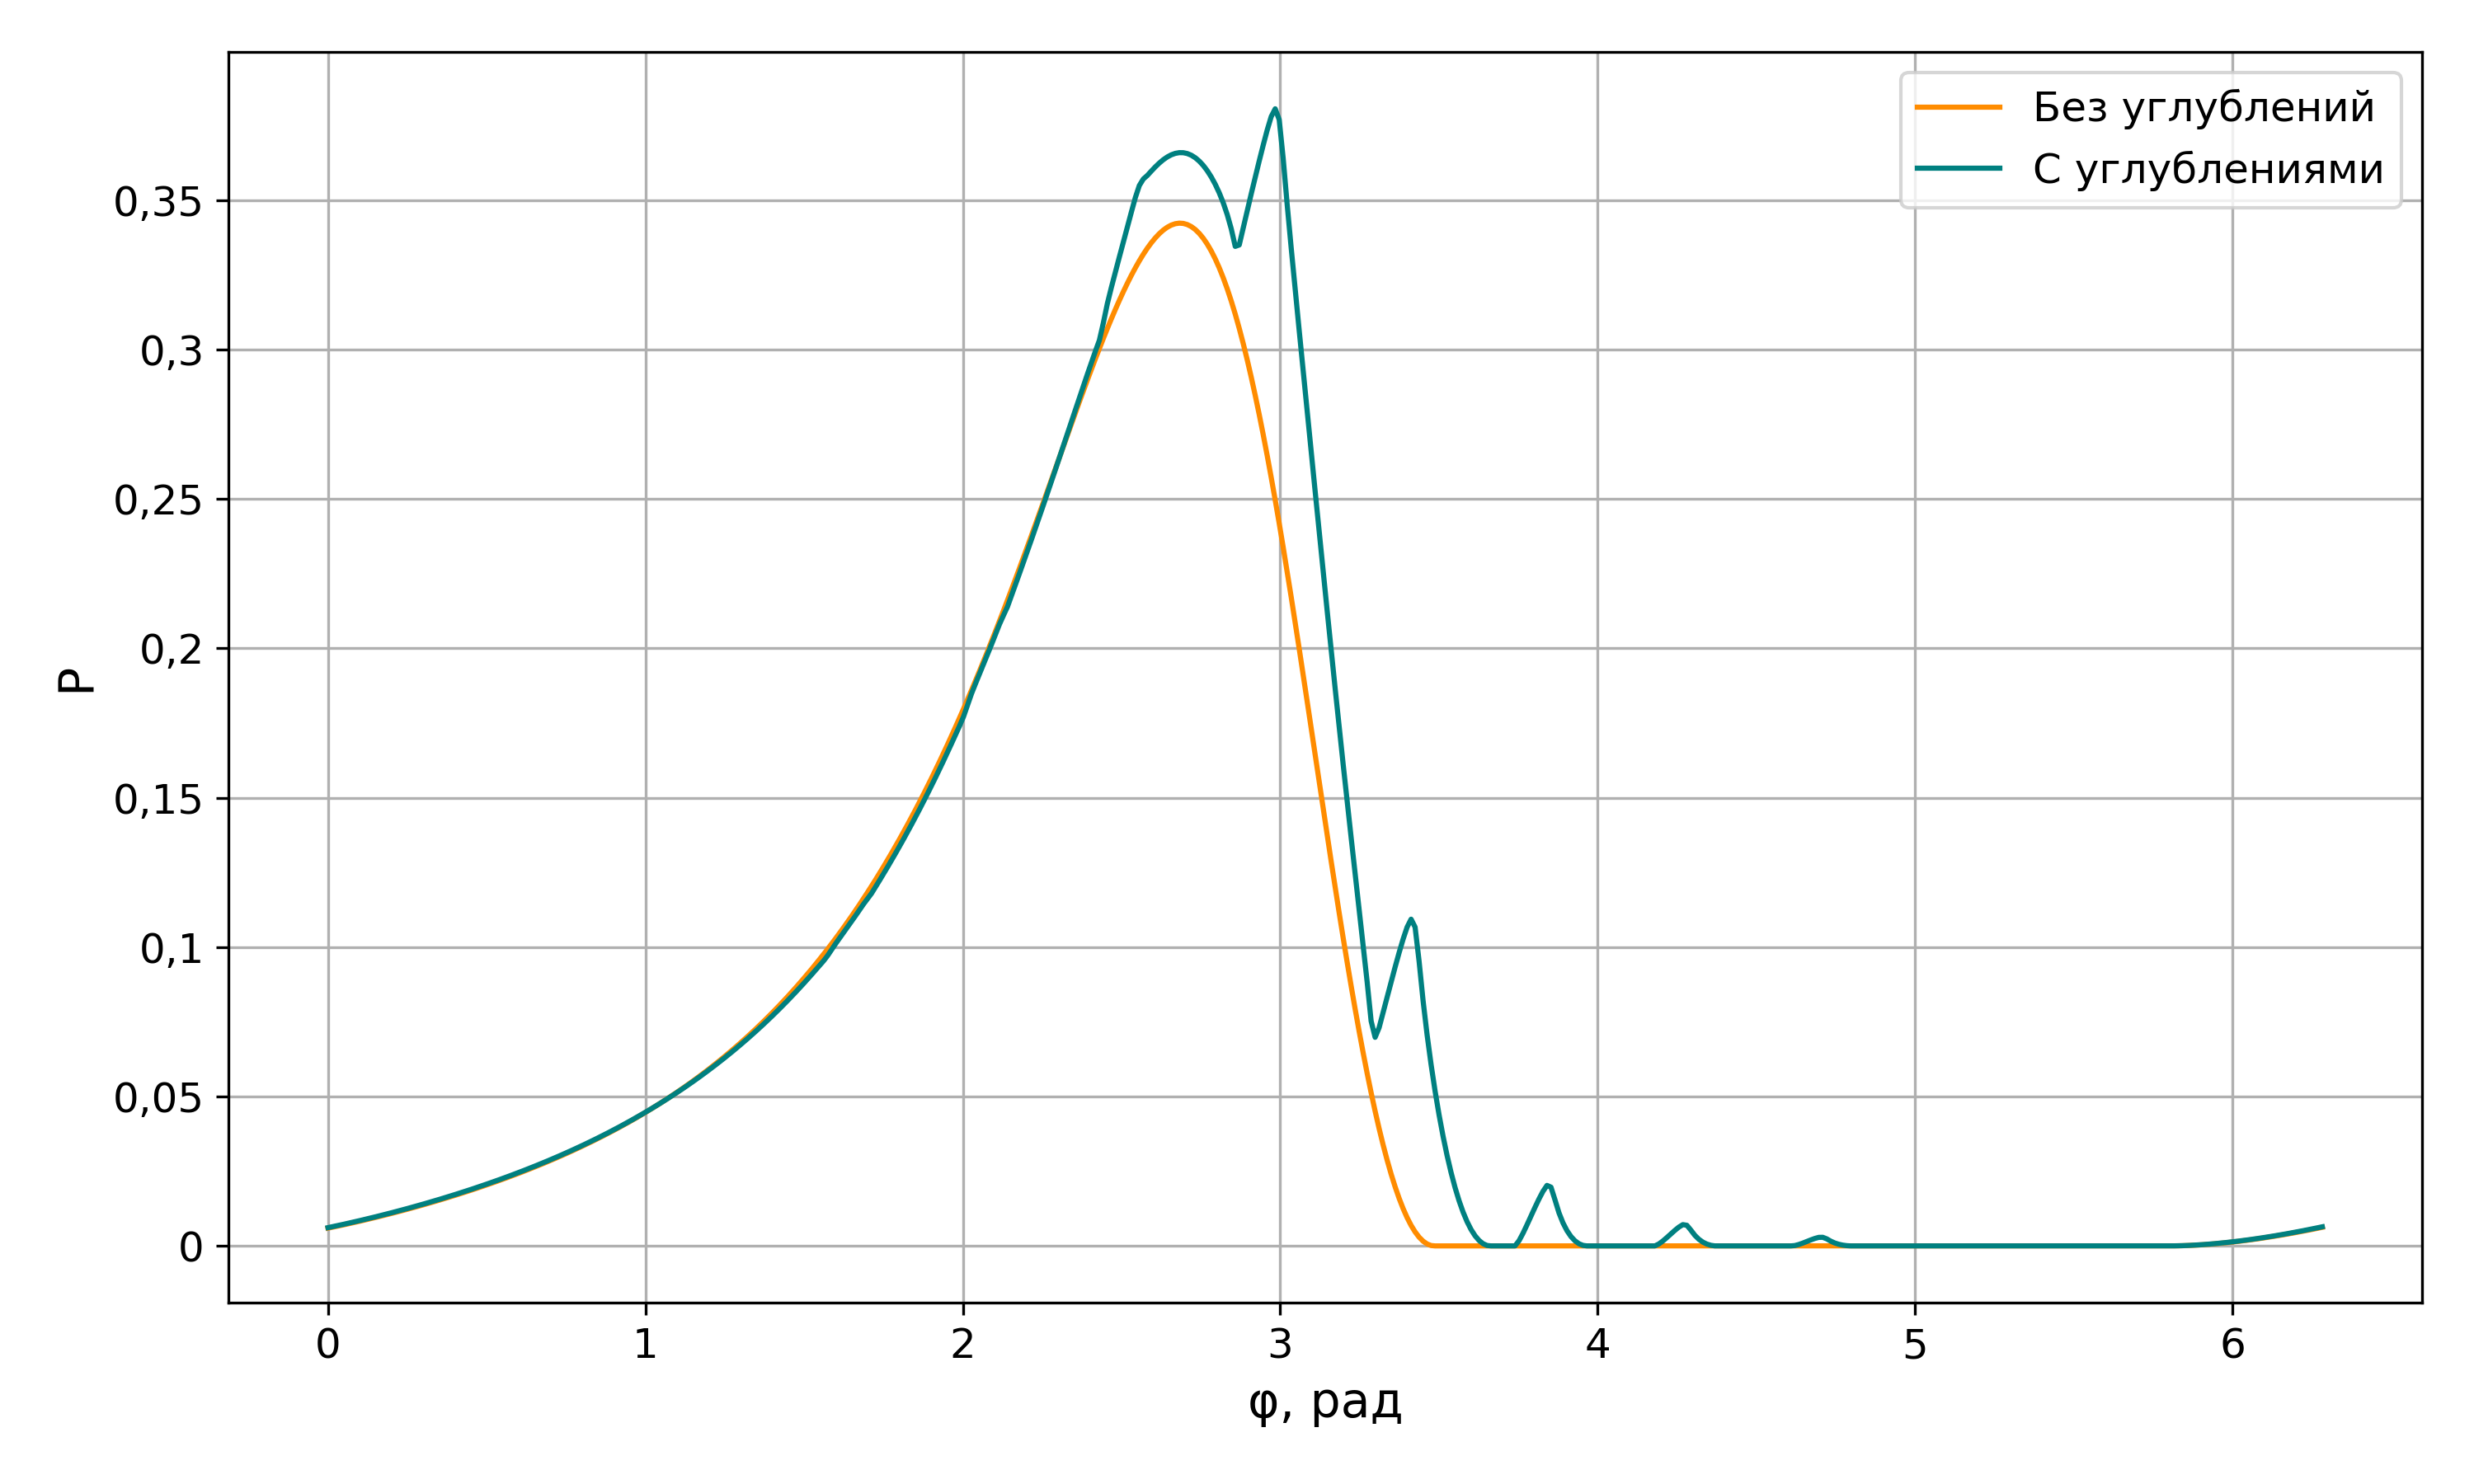
\includegraphics[width=\textwidth]{figures/pressure_2d.png}
\caption{Распределение давления $P(\varphi)$ при $Z=0$ для гладкого и текстурированного подшипников ($\varepsilon = 0{,}6$)}
\label{fig:pressure_2d}
\end{figure}

Для гладкого подшипника характерно наличие единственного максимума давления в области минимального зазора. Давление нарастает в сужающейся части зазора и обращается в нуль в расширяющейся части вследствие кавитации. При наличии микрорельефа на кривой давления появляются локальные возмущения, соответствующие углублениям.

На рисунке~\ref{fig:clearance_2d} показан профиль зазора $H(\varphi)$ в среднем сечении при $\varepsilon = 0{,}6$.

\begin{figure}[H]
\centering
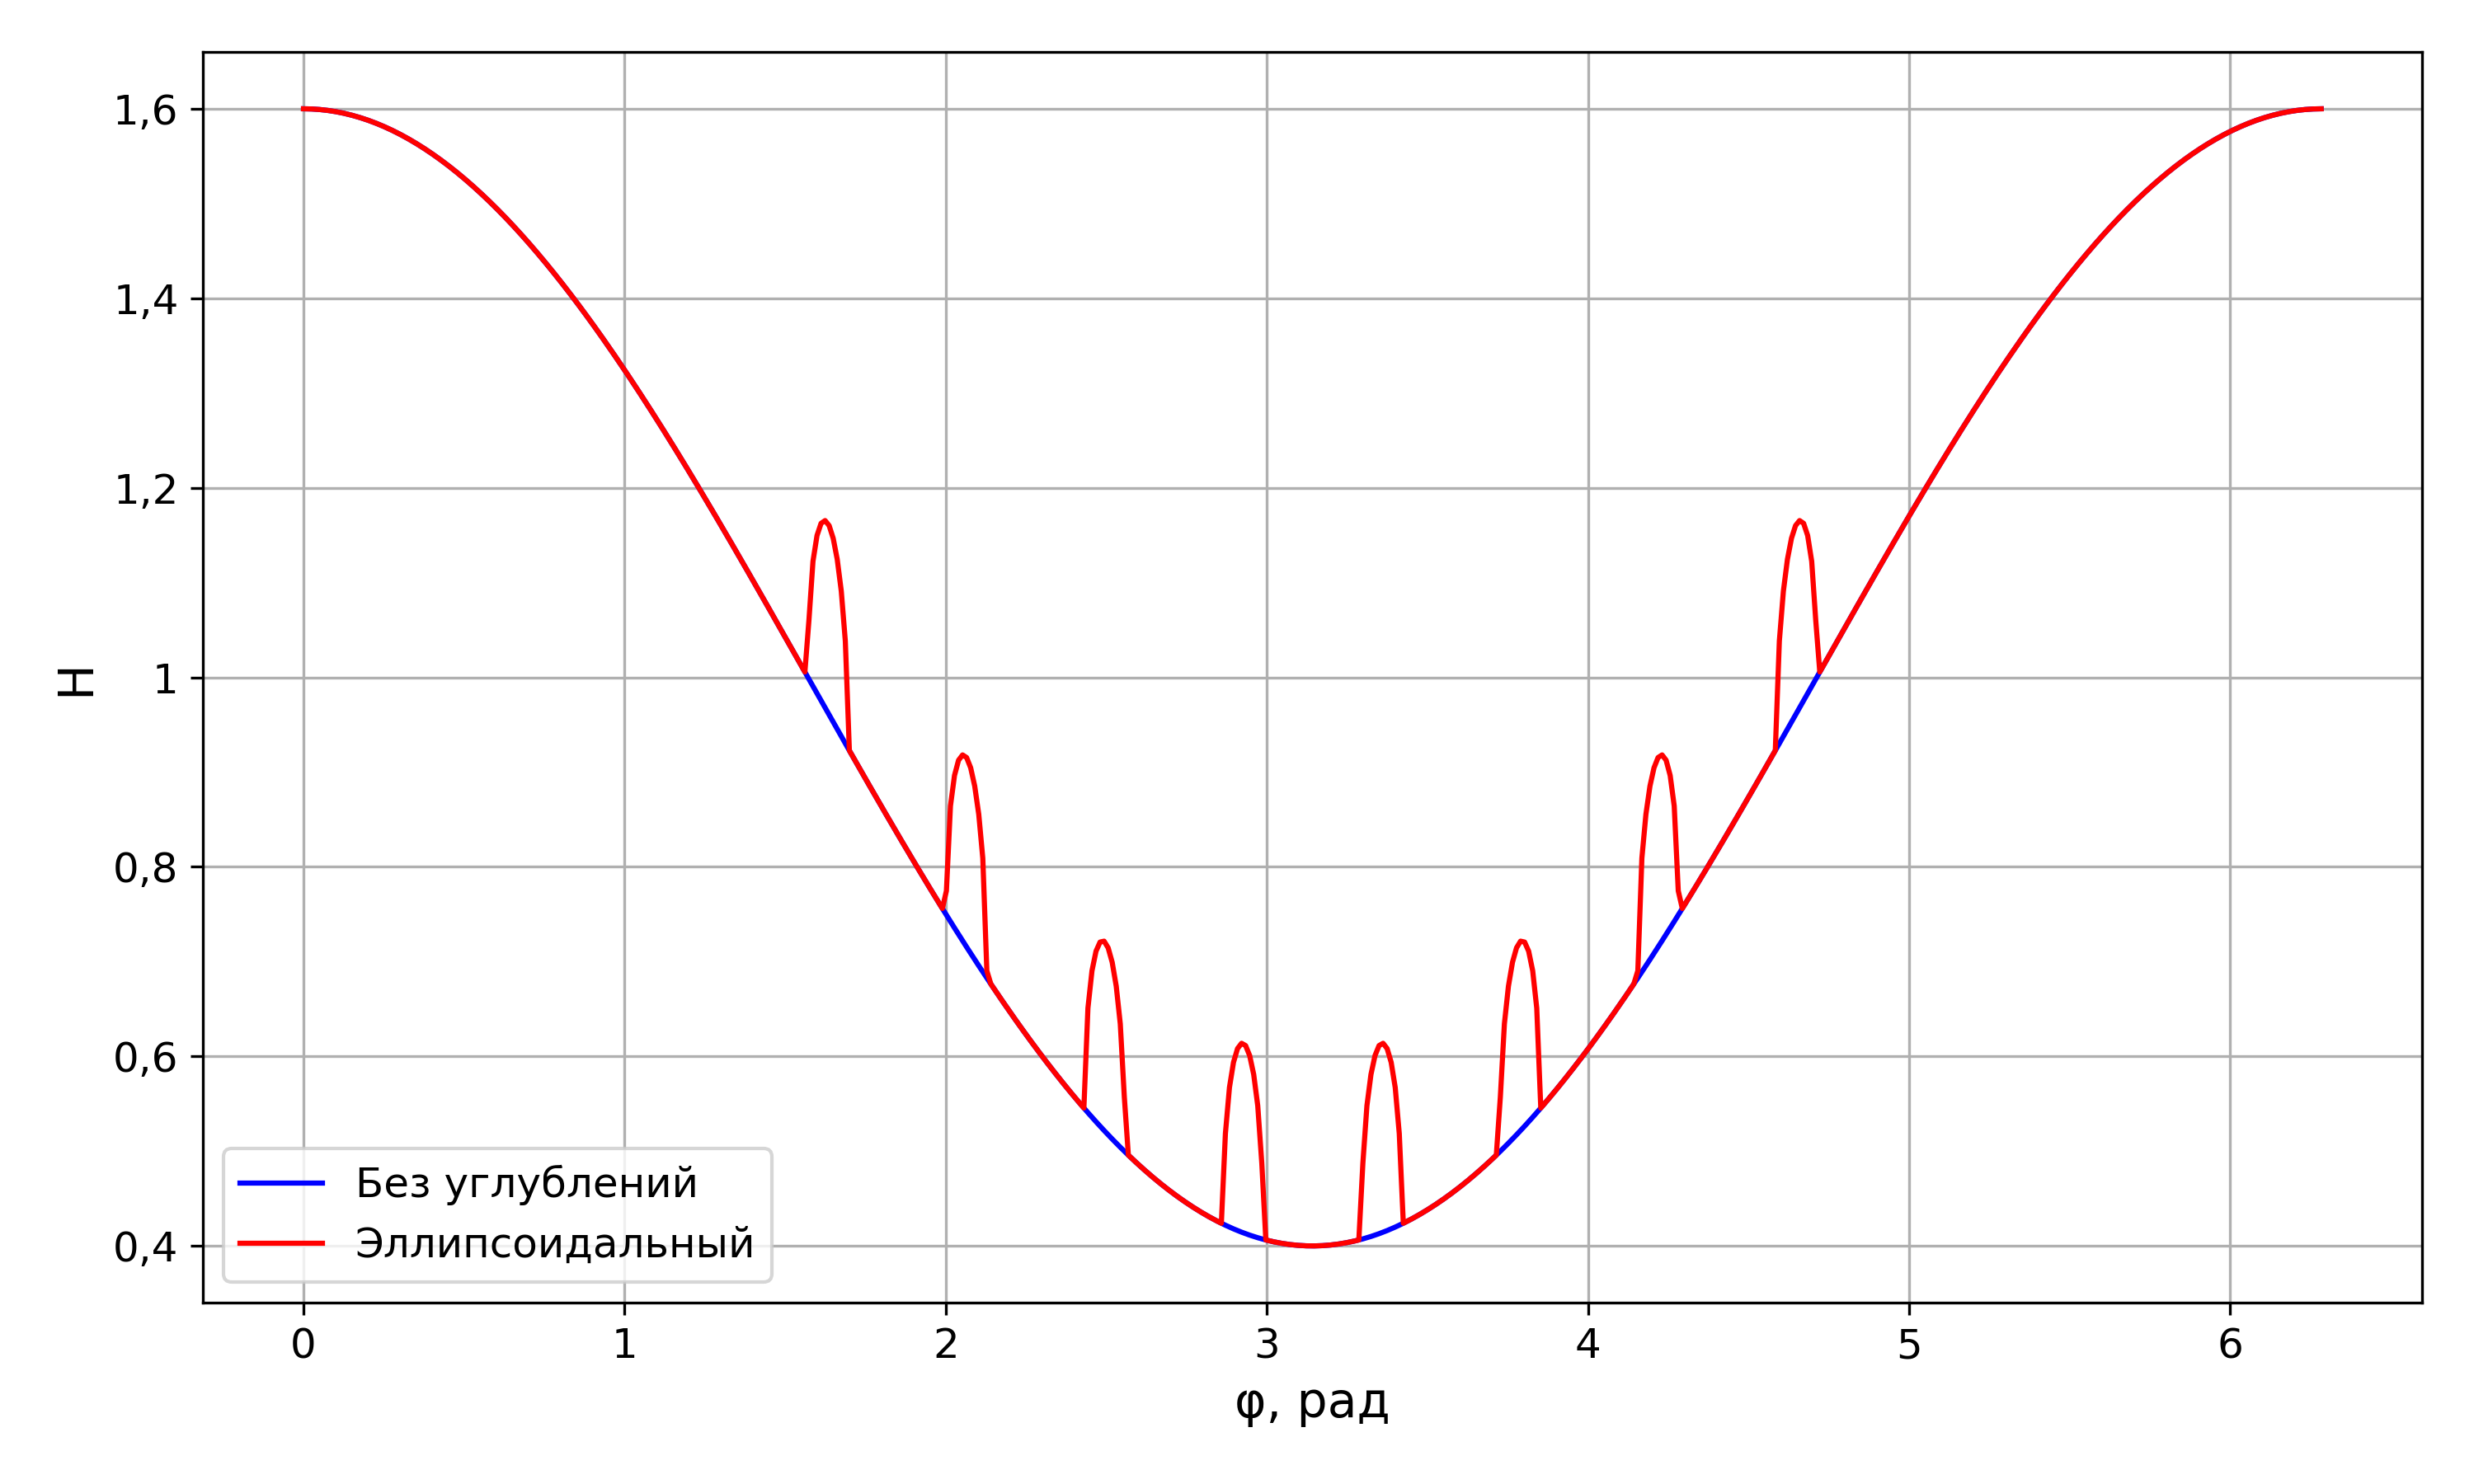
\includegraphics[width=\textwidth]{figures/clearance_2d.png}
\caption{Распределение зазора $H(\varphi)$ при $Z=0$ для подшипника с \varDimpleTypeGenitive{} углублениями ($\varepsilon = 0{,}6$)}
\label{fig:clearance_2d}
\end{figure}

На фоне плавного изменения зазора по закону $H = 1 + \varepsilon\cos\varphi$ наблюдаются локальные увеличения, соответствующие эллипсоидальным углублениям. Глубина каждого углубления составляет $\Delta H_{\max} = h_p/c = 0{,}2$ в безразмерных единицах.

Трёхмерные распределения зазора и давления при $\varepsilon = 0{,}6$ представлены на рисунках~\ref{fig:clearance_3d} и~\ref{fig:pressure_3d}.

\begin{figure}[H]
\centering
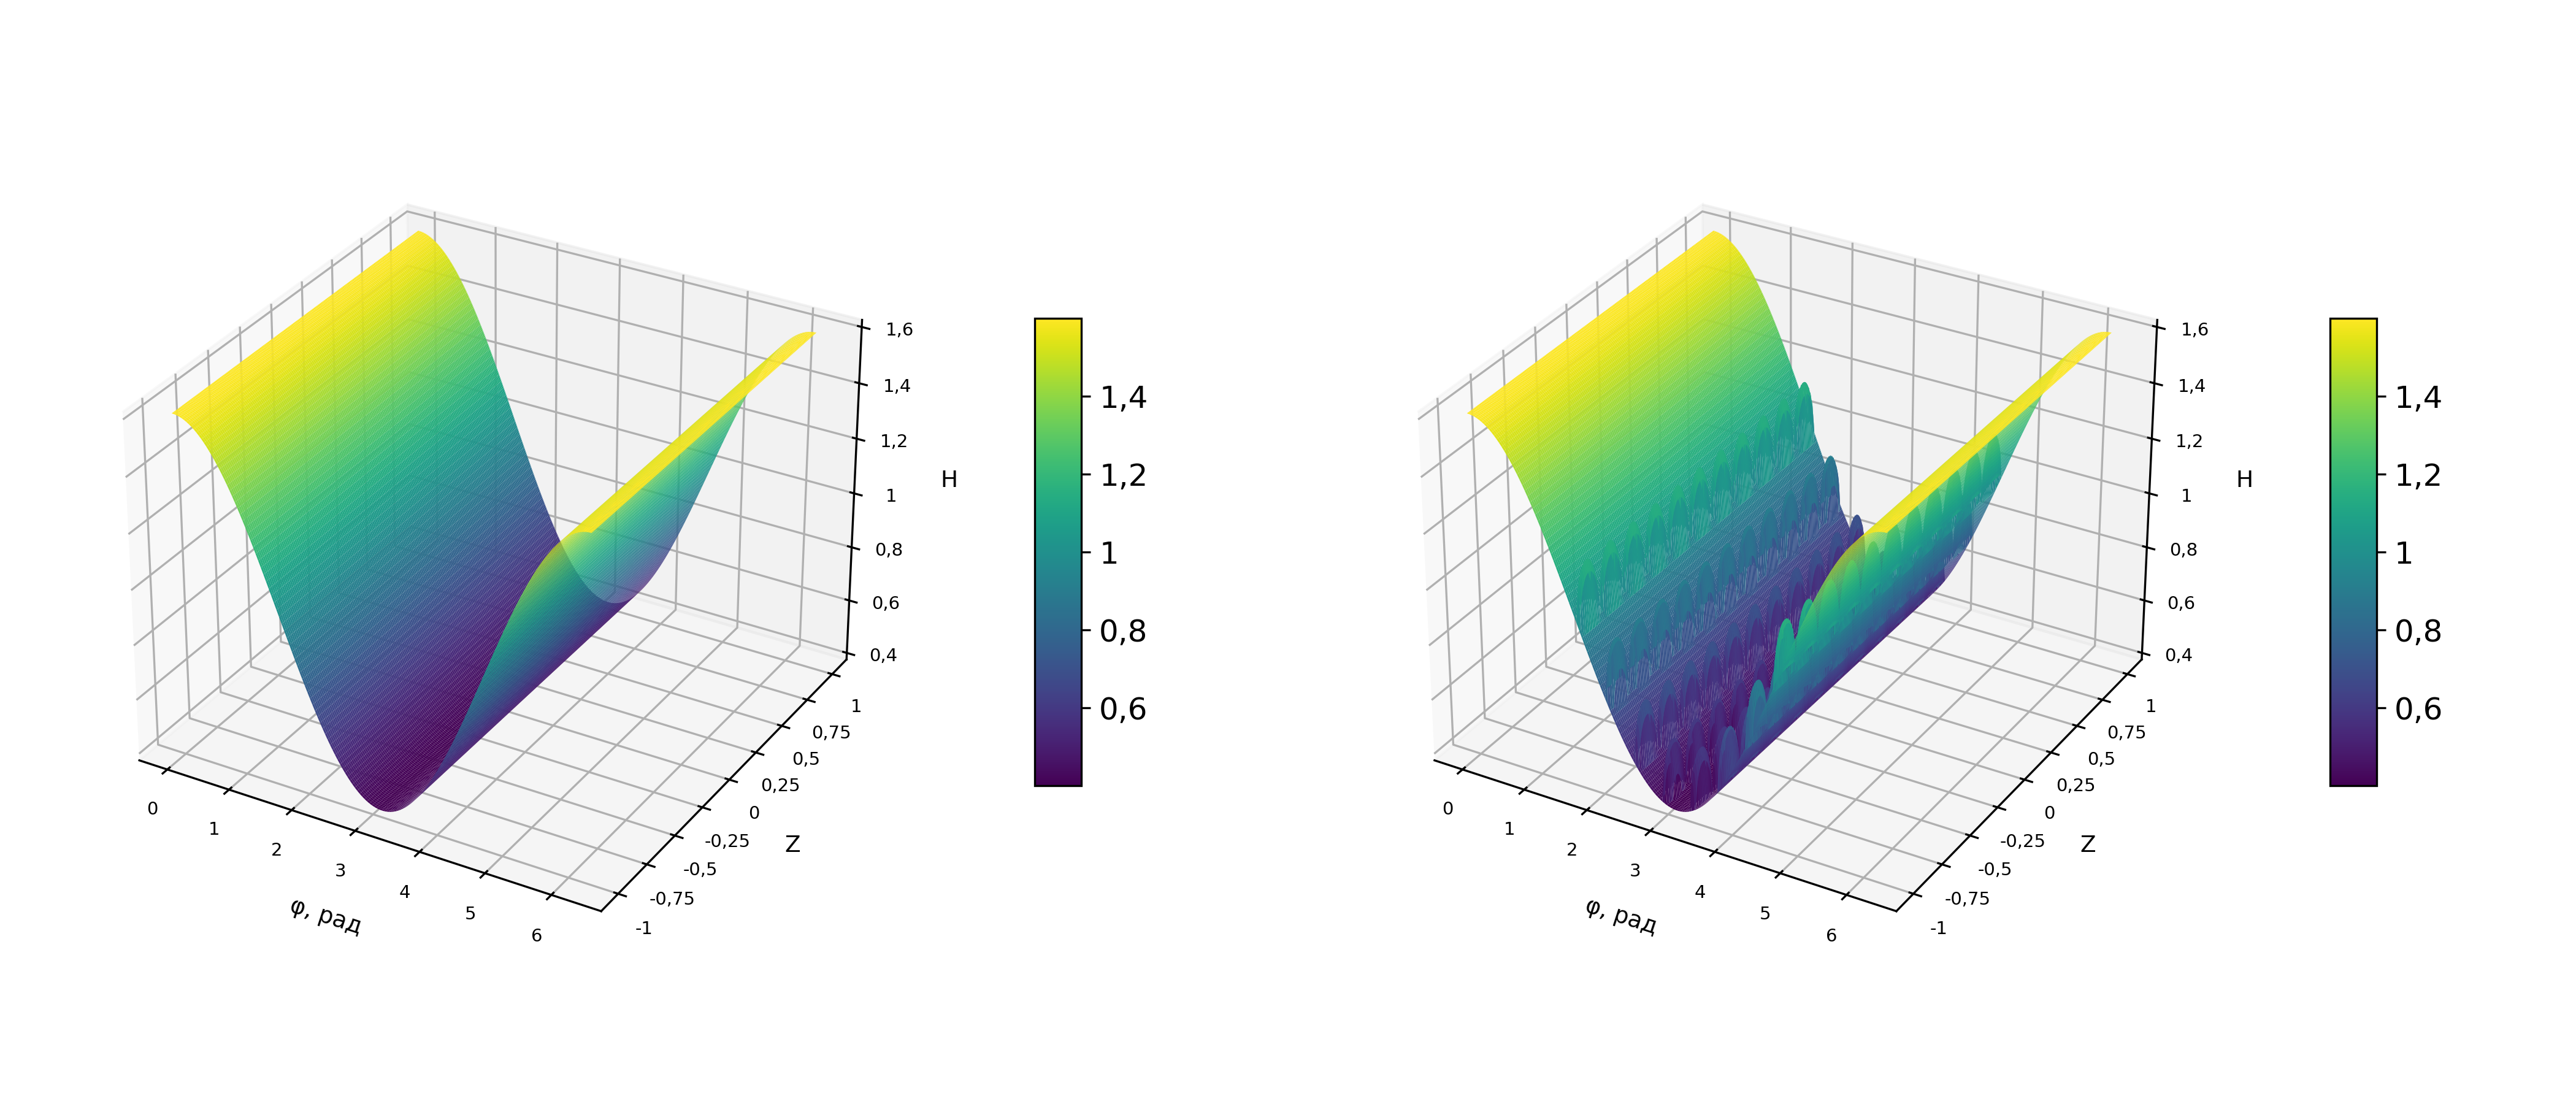
\includegraphics[width=\textwidth]{figures/clearance_3d.png}
\caption{Трёхмерное распределение зазора $H(\varphi, Z)$ ($\varepsilon = 0{,}6$)}
\label{fig:clearance_3d}
\end{figure}

На рисунке~\ref{fig:clearance_3d} отчётливо видна регулярная структура микрорельефа: 8 углублений по окружности и 11 рядов по длине подшипника в зоне $90^\circ - 270^\circ$.

\begin{figure}[H]
\centering
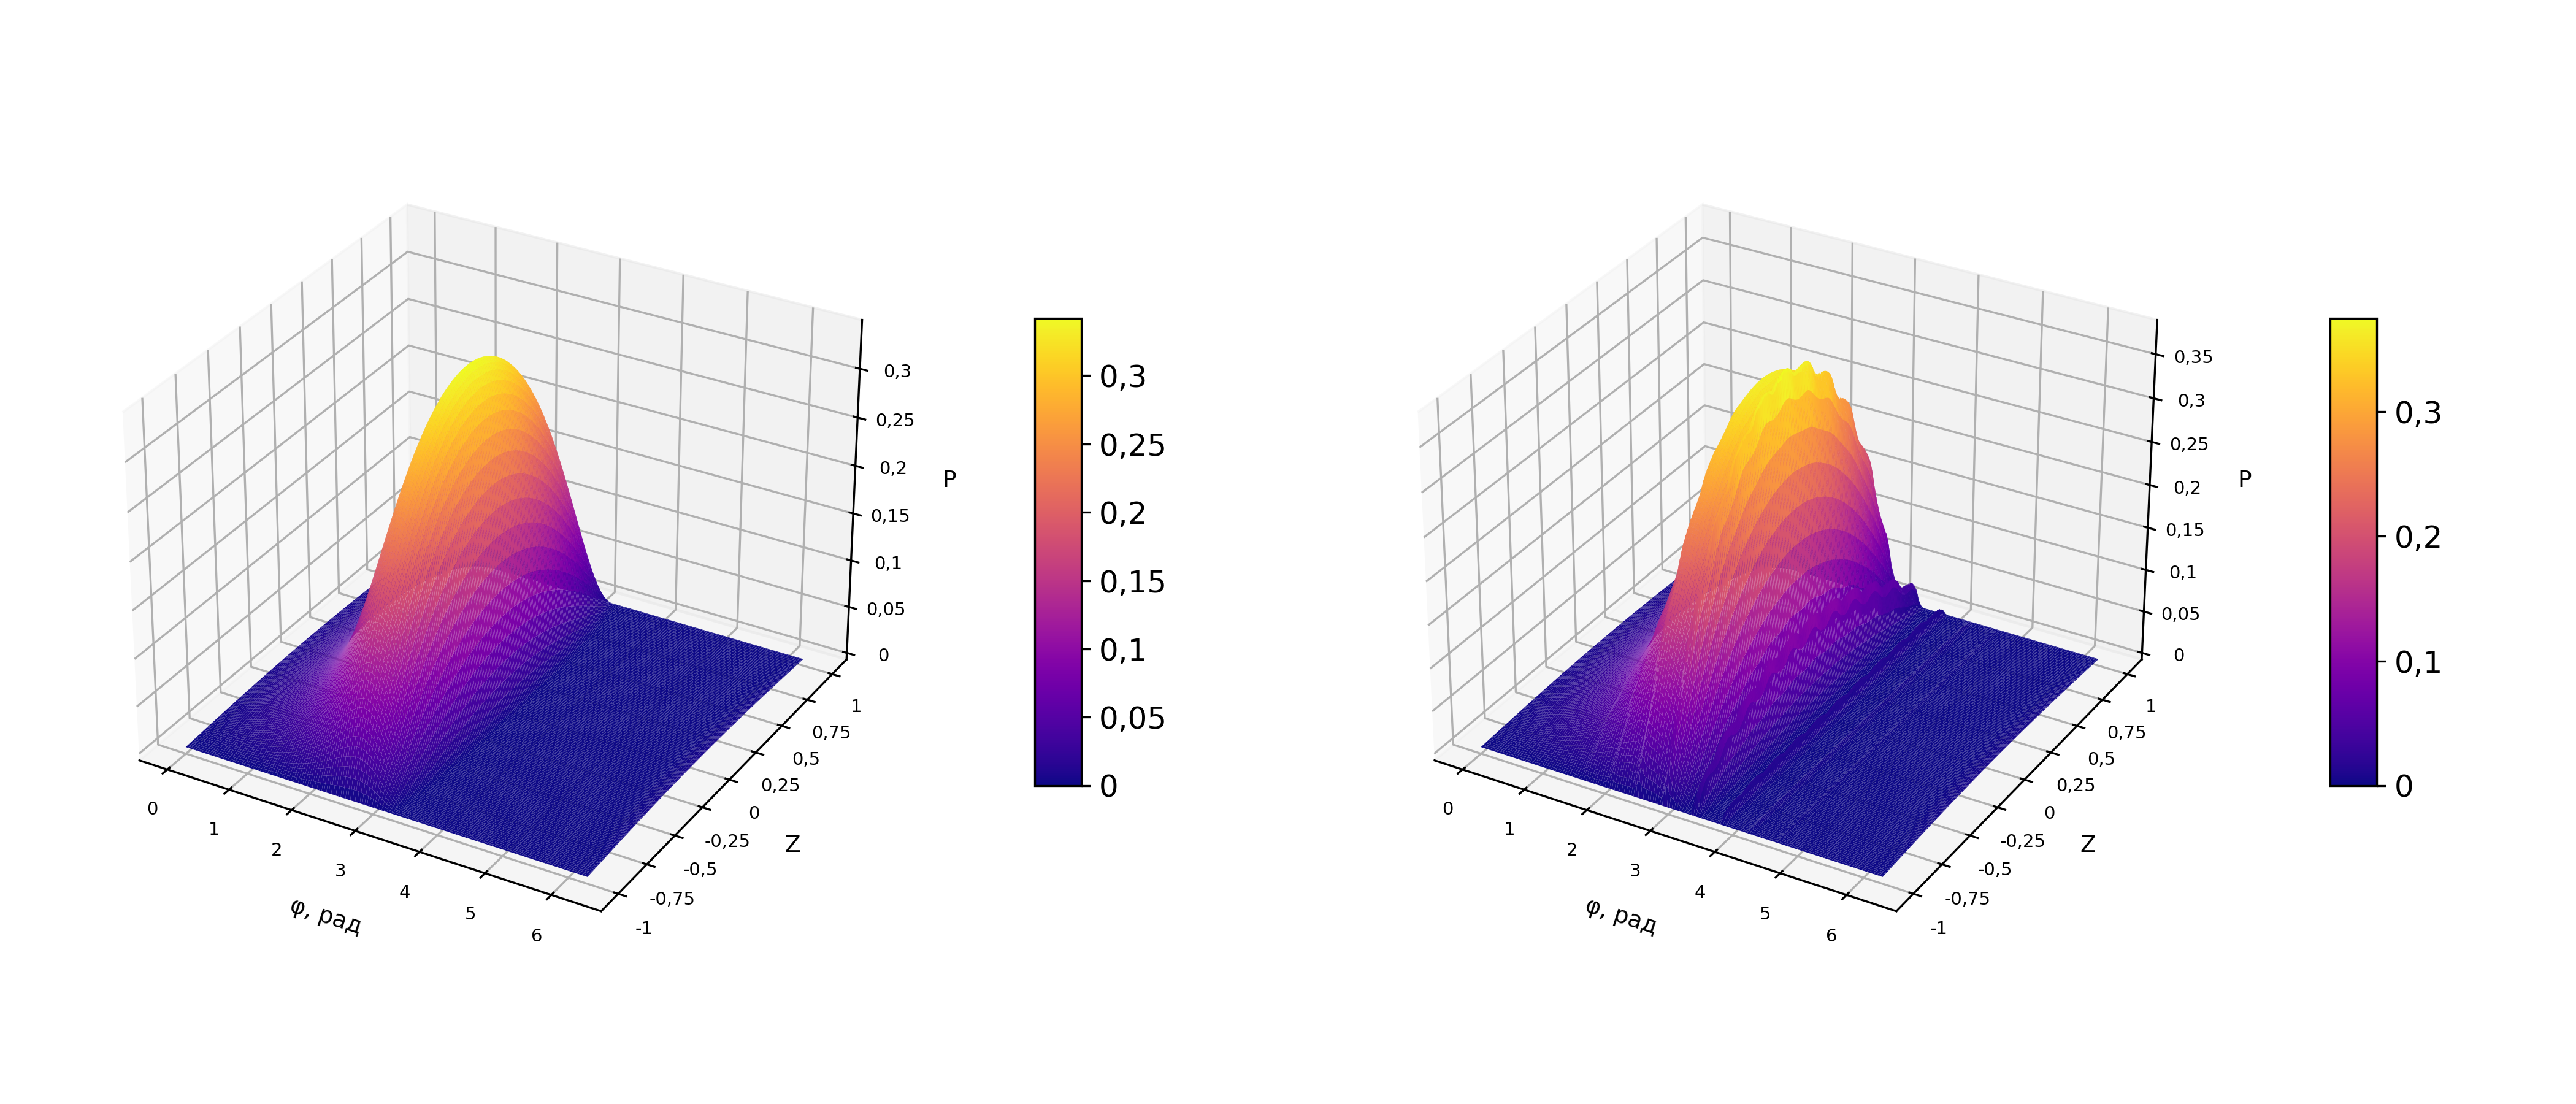
\includegraphics[width=\textwidth]{figures/pressure_3d.png}
\caption{Трёхмерное распределение давления $P(\varphi, Z)$ ($\varepsilon = 0{,}6$)}
\label{fig:pressure_3d}
\end{figure}

На рисунке~\ref{fig:pressure_3d} помимо основного максимума давления наблюдаются локальные возмущения на каждом углублении. На входной кромке углубления зазор сужается, что создаёт дополнительный подъём давления -- микрогидродинамический эффект. На выходной кромке давление снижается, однако благодаря кавитационному ограничению ($P \geq 0$) суммарный вклад каждого углубления в несущую способность положителен.

\subsection{Сравнительный анализ интегральных показателей}

Интегральные характеристики гладкого подшипника и подшипника с эллипсоидальными углублениями для выбранных значений эксцентриситета представлены в таблицах~\ref{tab:smooth_results} и~\ref{tab:textured_results}.

\begin{table}[H]
\small
\centering
\caption{Характеристики гладкого подшипника}
\label{tab:smooth_results}
\begin{tabular}{|c|c|c|c|}
\hline
$\boldsymbol{\varepsilon}$ & $\boldsymbol{F}$\textbf{, Н} & $\boldsymbol{\mu}$ & $\boldsymbol{Q}$\textbf{, л/с} \\
\hline
0{,}05 & 259{,}5 & 0{,}2291 & 0{,}2398 \\
\hline
0{,}16 & 835{,}7 & 0{,}0722 & 0{,}2395 \\
\hline
0{,}26 & 1478{,}5 & 0{,}0420 & 0{,}2389 \\
\hline
0{,}37 & 2261{,}3 & 0{,}0287 & 0{,}2380 \\
\hline
0{,}48 & 3286{,}8 & 0{,}0211 & 0{,}2370 \\
\hline
0{,}59 & 4764{,}4 & 0{,}0160 & 0{,}2360 \\
\hline
0{,}69 & 7222{,}5 & 0{,}0120 & 0{,}2351 \\
\hline
0{,}80 & 12218{,}3 & 0{,}0087 & 0{,}2344 \\
\hline
\end{tabular}
\end{table}

\begin{table}[H]
\small
\centering
\caption{Характеристики подшипника с \varDimpleTypeGenitive{} углублениями}
\label{tab:textured_results}
\begin{tabular}{|c|c|c|c|}
\hline
$\boldsymbol{\varepsilon}$ & $\boldsymbol{F}$\textbf{, Н} & $\boldsymbol{\mu}$ & $\boldsymbol{Q}$\textbf{, л/с} \\
\hline
0{,}05 & 362{,}1 & 0{,}1623 & 0{,}2433 \\
\hline
0{,}16 & 922{,}3 & 0{,}0645 & 0{,}2429 \\
\hline
0{,}26 & 1586{,}0 & 0{,}0386 & 0{,}2423 \\
\hline
0{,}37 & 2415{,}6 & 0{,}0265 & 0{,}2415 \\
\hline
0{,}48 & 3527{,}4 & 0{,}0193 & 0{,}2405 \\
\hline
0{,}59 & 5252{,}3 & 0{,}0142 & 0{,}2394 \\
\hline
0{,}69 & 8491{,}3 & 0{,}0100 & 0{,}2384 \\
\hline
0{,}80 & 17139{,}1 & 0{,}0060 & 0{,}2374 \\
\hline
\end{tabular}
\end{table}

Нагрузочная способность $F$ нелинейно возрастает с увеличением эксцентриситета для обоих вариантов подшипника. Текстурированный подшипник обладает большей нагрузочной способностью при всех значениях $\varepsilon$. При высоких эксцентриситетах ($\varepsilon = 0{,}80$) эффект текстурирования выражен наиболее ярко: нагрузочная способность текстурированного подшипника (17139{,}1~Н) превышает гладкий аналог (12218{,}3~Н) на 40{,}3\%.

Коэффициент трения $\mu$ монотонно убывает при увеличении $\varepsilon$ и для текстурированного подшипника ниже при всех значениях эксцентриситета. Расход смазки $Q$ слабо зависит от $\varepsilon$ и у текстурированного подшипника несколько выше за счёт увеличения эффективного объёма смазочного слоя в зоне углублений.

Для количественной оценки эффективности текстурирования в таблице~\ref{tab:comparison} представлены результаты сравнения при $\varepsilon = 0{,}6$.

\begin{table}[H]
\small
\centering
\caption{Сравнение характеристик при $\varepsilon = 0{,}6$}
\label{tab:comparison}
\begin{tabular}{|l|c|c|c|}
\hline
\textbf{Характеристика} & \textbf{Гладкий} & \textbf{С углублениями} & $\boldsymbol{\Delta}$\textbf{, \%} \\
\hline
Нагрузка $F$, Н & 5028{,}5 & 5572{,}7 & $+10{,}82$ \\
\hline
Коэфф. трения $\mu$ & 0{,}01538 & 0{,}01356 & $-11{,}78$ \\
\hline
Расход $Q$, л/с & 0{,}2359 & 0{,}2392 & $+1{,}43$ \\
\hline
\end{tabular}
\end{table}

Нанесение эллипсоидальных углублений увеличивает несущую способность подшипника на 10{,}82\% за счёт микрогидродинамического эффекта. Коэффициент трения снижается на 11{,}78\% вследствие увеличения средней толщины смазочного слоя в зоне углублений. Расход смазки возрастает на 1{,}43\%, что способствует улучшению теплоотвода без существенного увеличения требуемой производительности системы маслоснабжения.

На рисунках~\ref{fig:load_vs_eps}-\ref{fig:flow_vs_eps} представлены зависимости интегральных характеристик от эксцентриситета для обоих вариантов подшипника.

\begin{figure}[H]
\centering
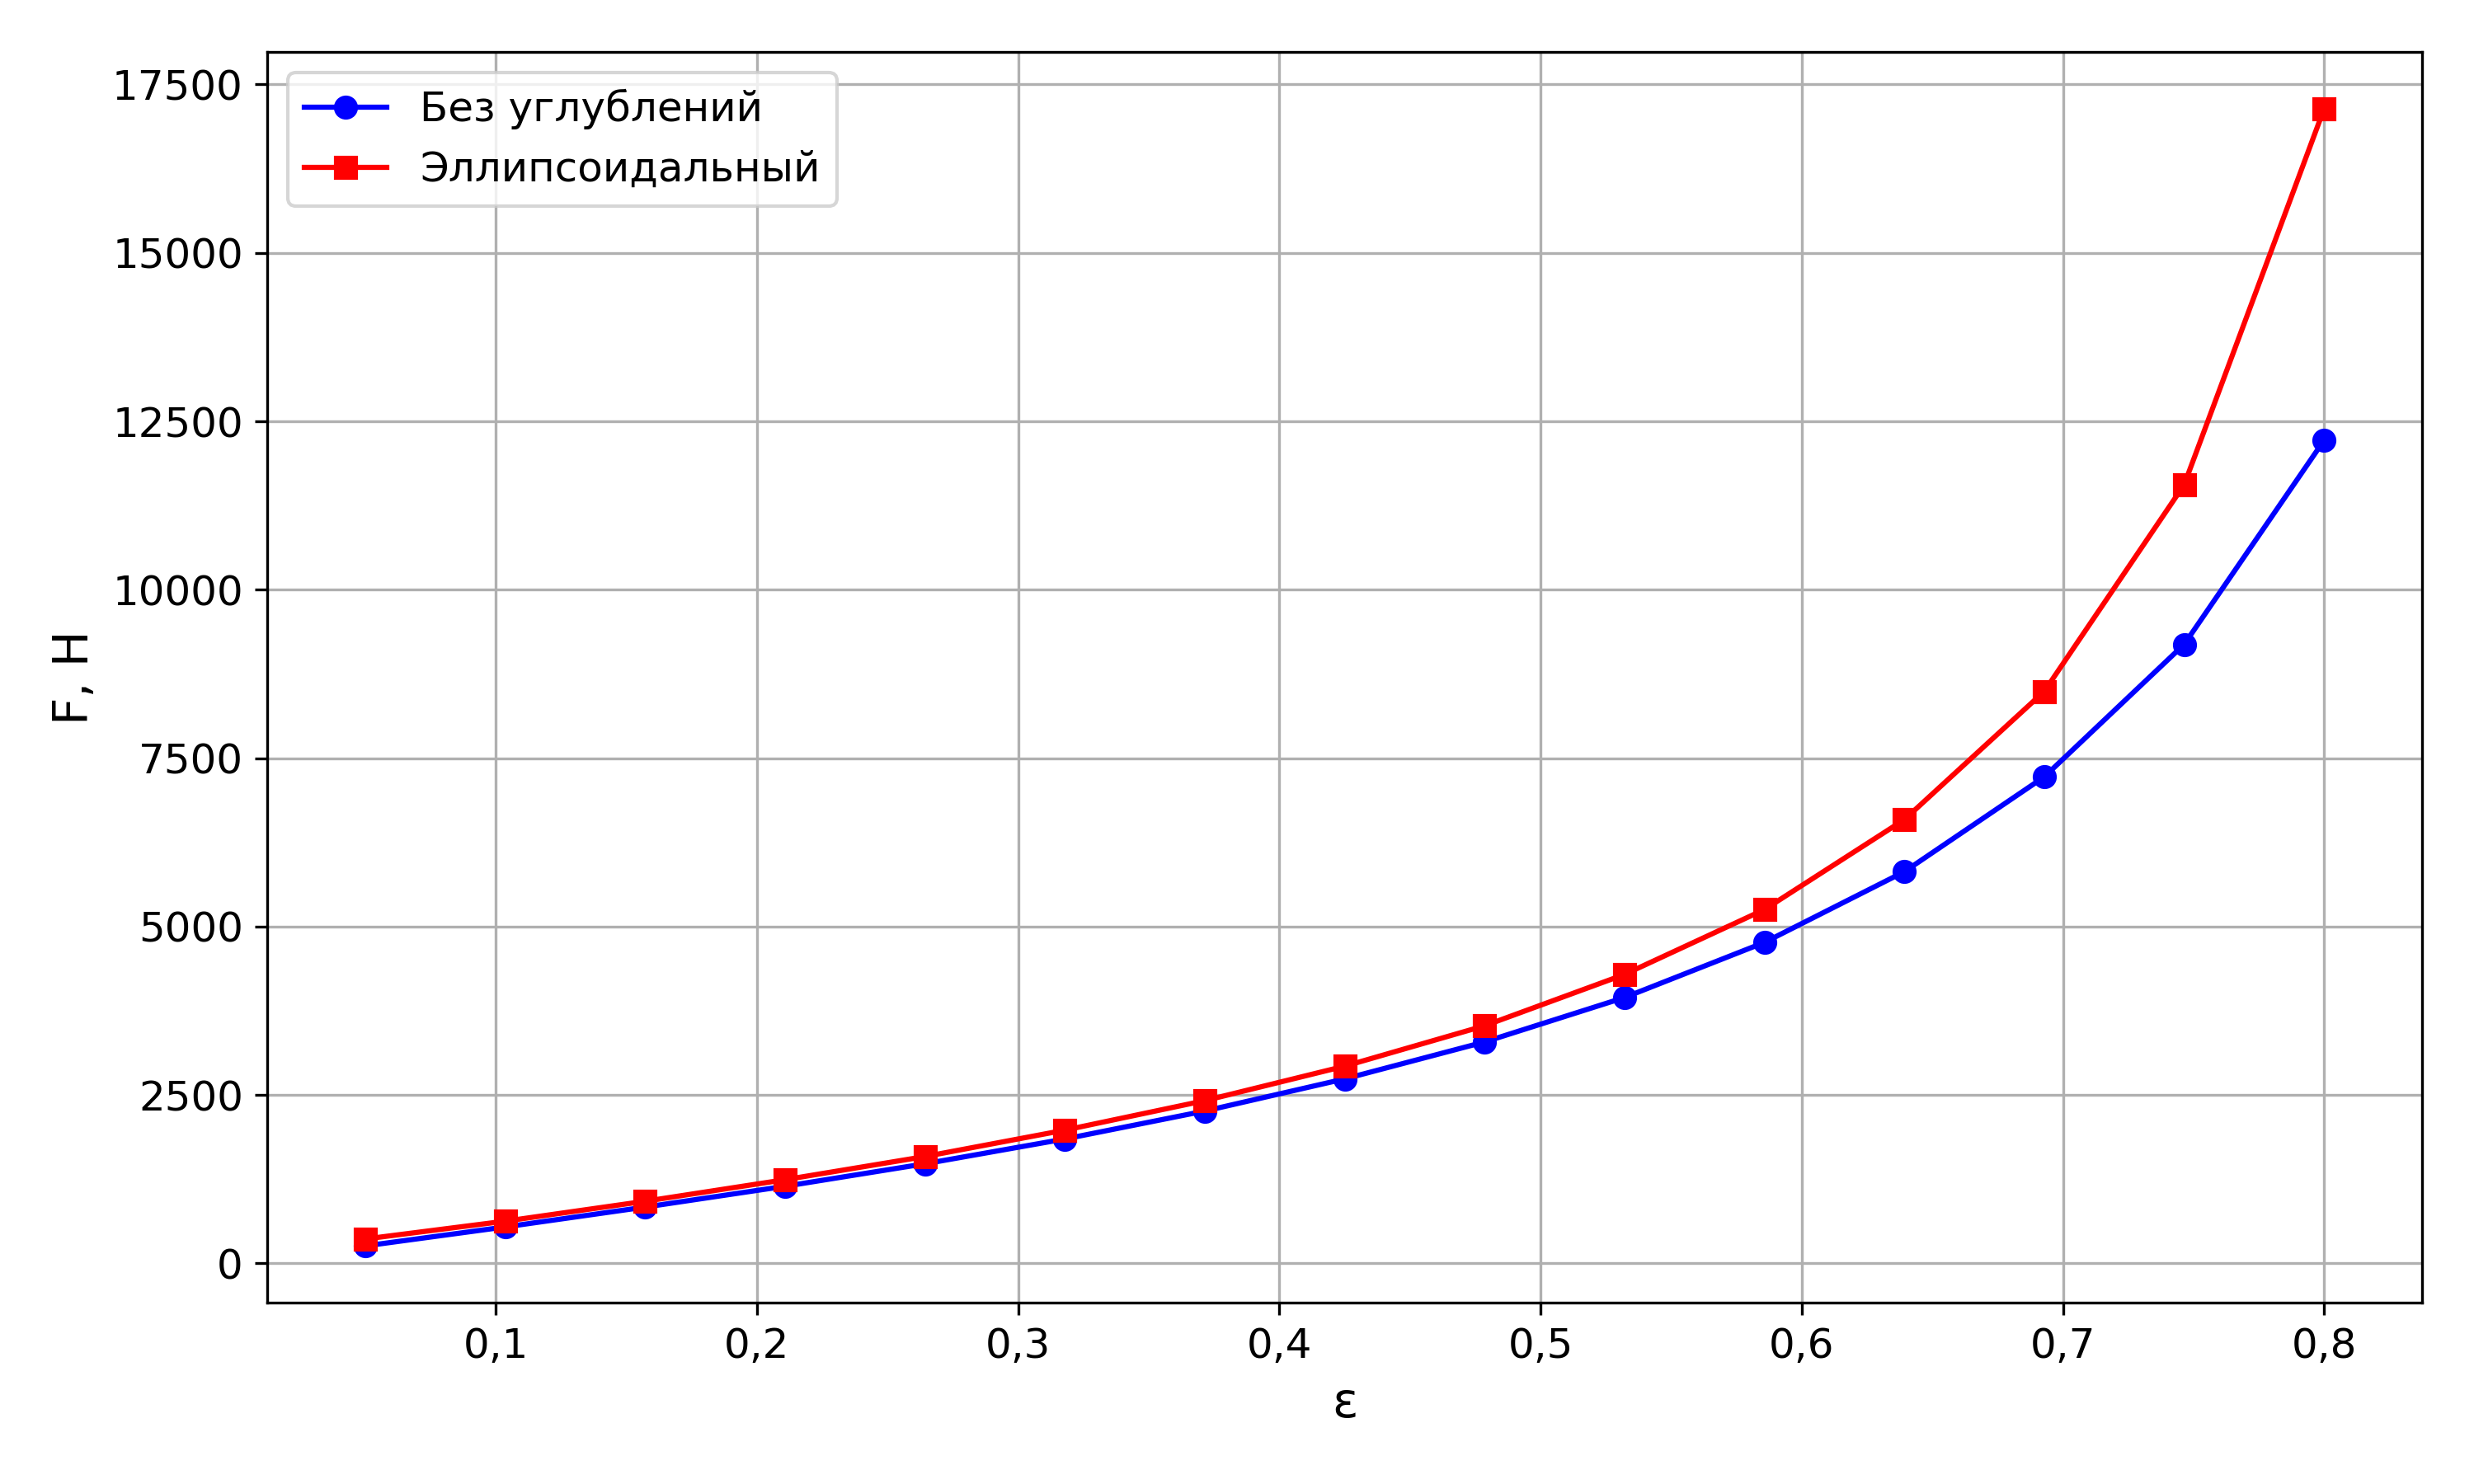
\includegraphics[width=\textwidth]{figures/load_vs_epsilon.png}
\caption{Нагрузочная способность $F(\varepsilon)$ для гладкого и текстурированного подшипников}
\label{fig:load_vs_eps}
\end{figure}

Кривая $F(\varepsilon)$ для текстурированного подшипника проходит выше во всём диапазоне эксцентриситетов. С ростом $\varepsilon$ разрыв между кривыми увеличивается, что обусловлено степенной зависимостью давления от толщины зазора.

\begin{figure}[H]
\centering
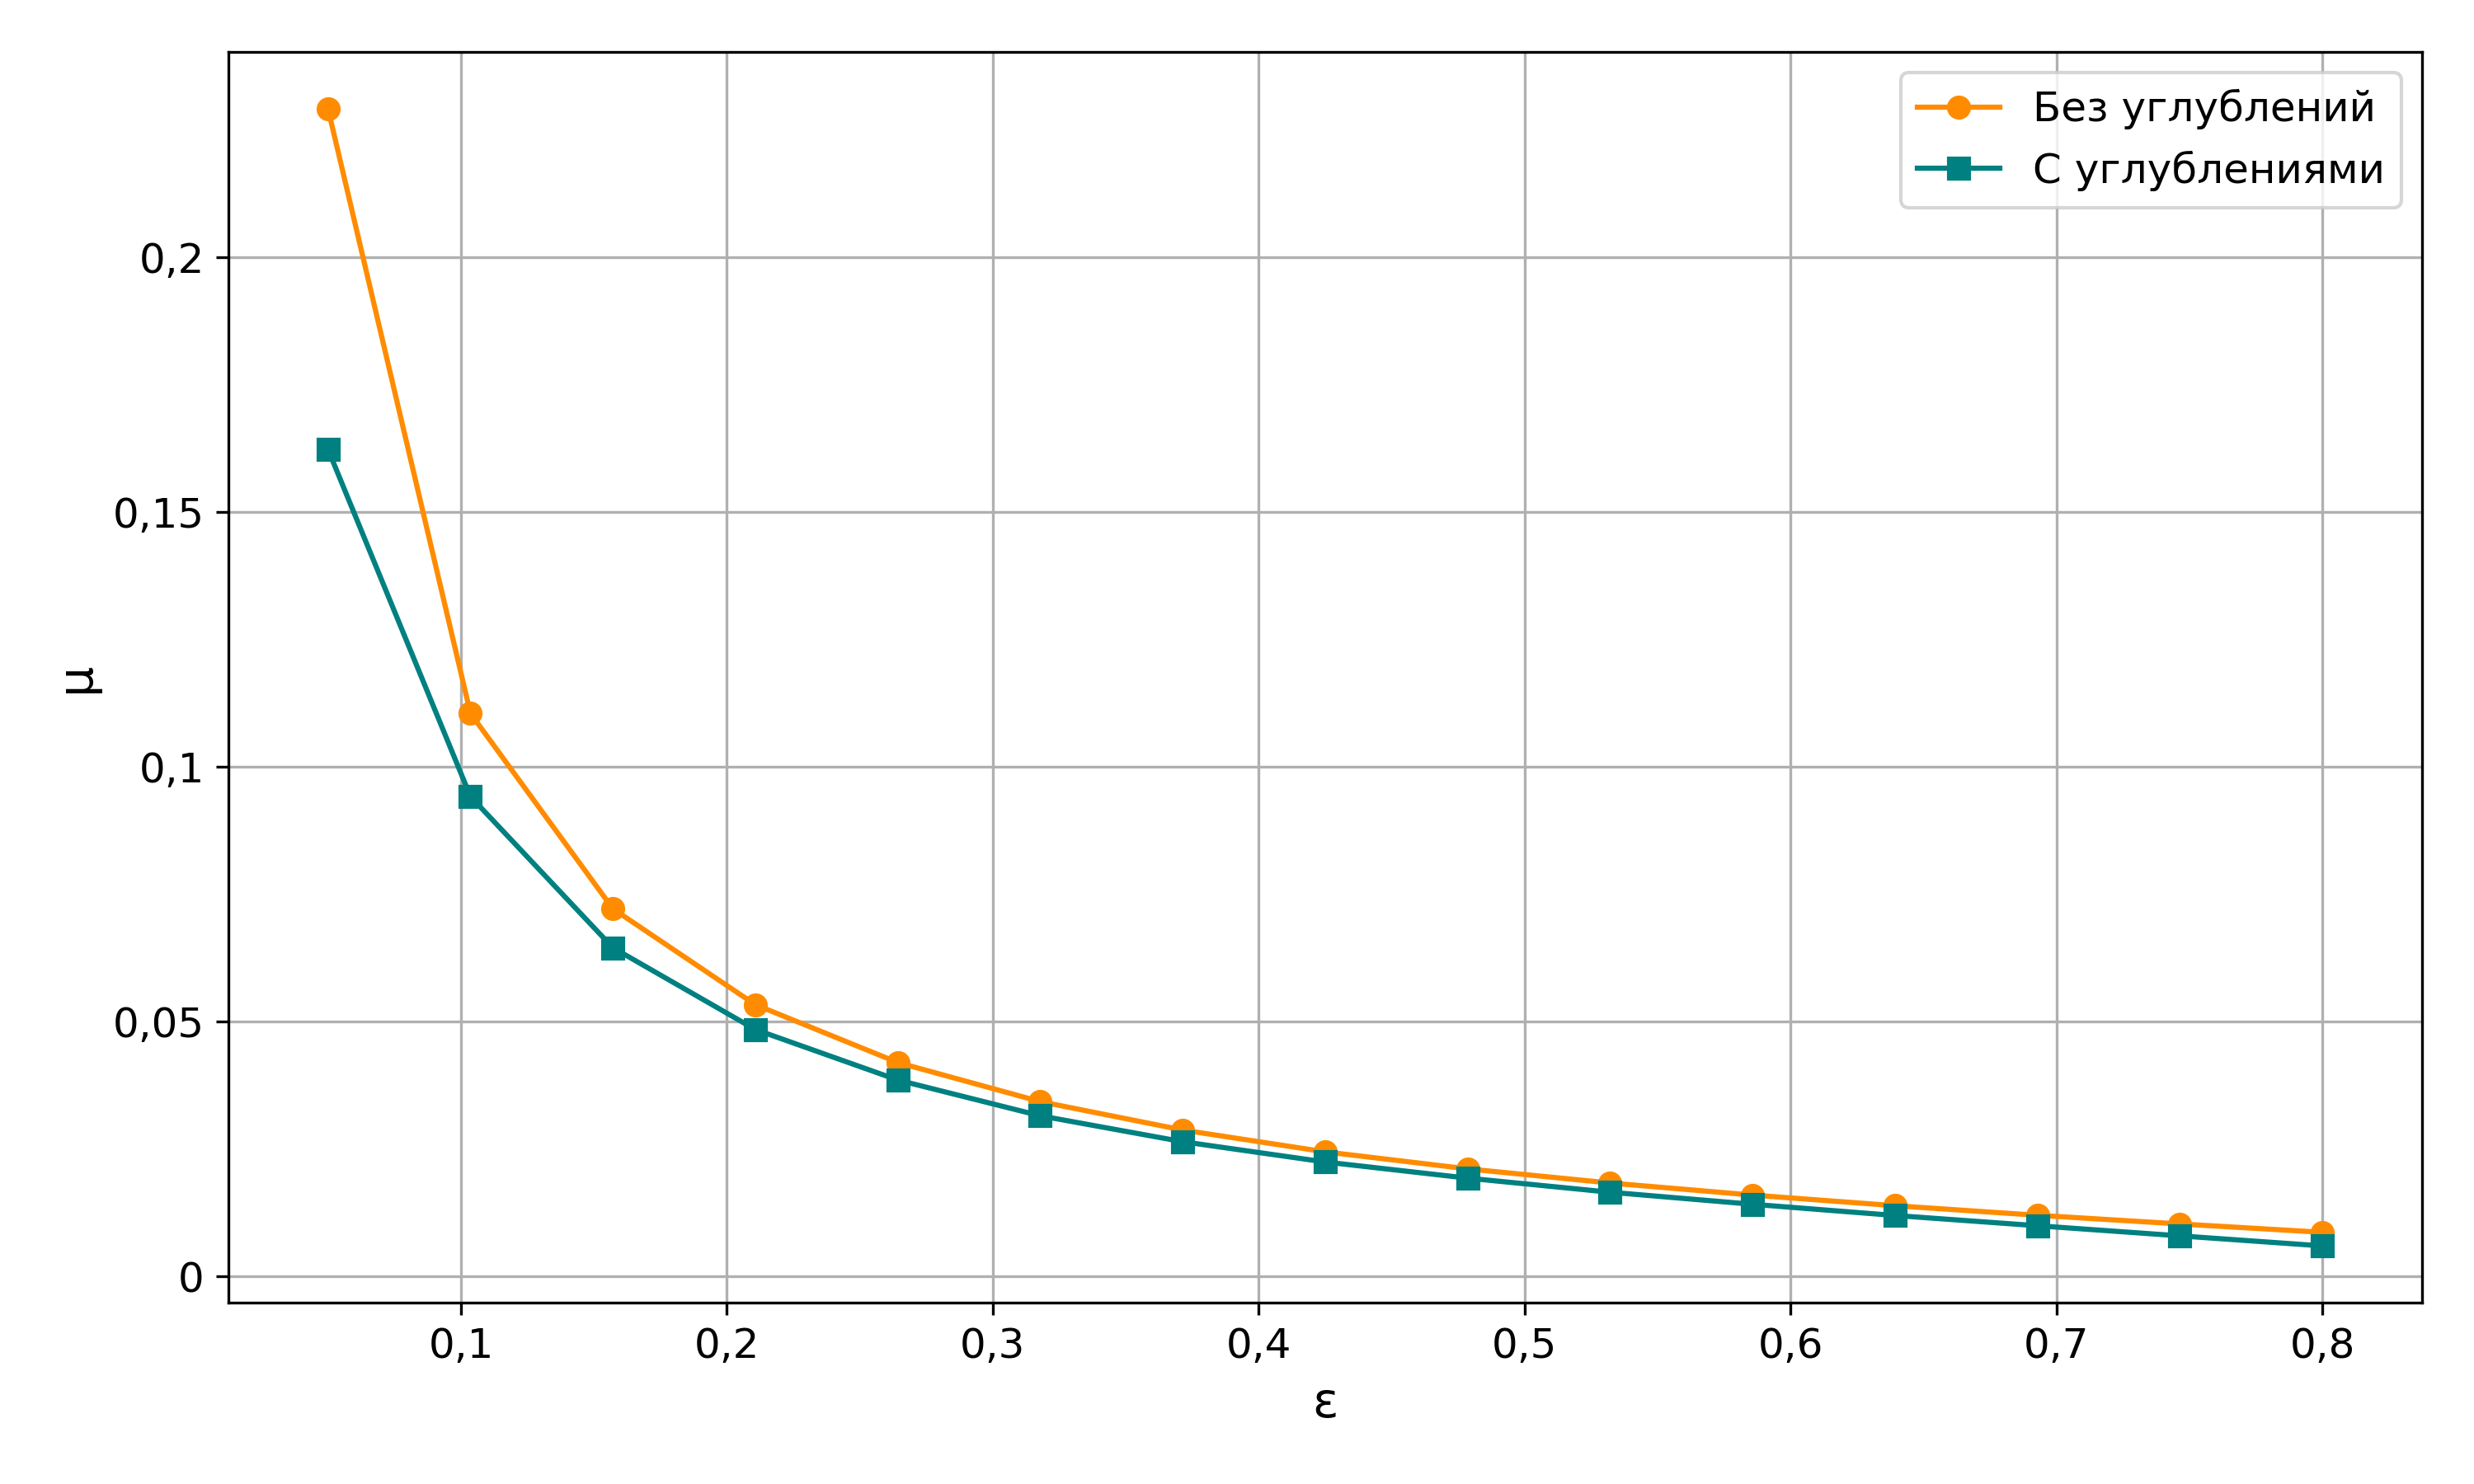
\includegraphics[width=\textwidth]{figures/friction_vs_epsilon.png}
\caption{Коэффициент трения $\mu(\varepsilon)$ для гладкого и текстурированного подшипников}
\label{fig:friction_vs_eps}
\end{figure}

Коэффициент трения текстурированного подшипника ниже гладкого при всех значениях $\varepsilon$. Обе кривые монотонно убывают. В относительном выражении снижение трения сопоставимо во всём диапазоне эксцентриситетов.

\begin{figure}[H]
\centering
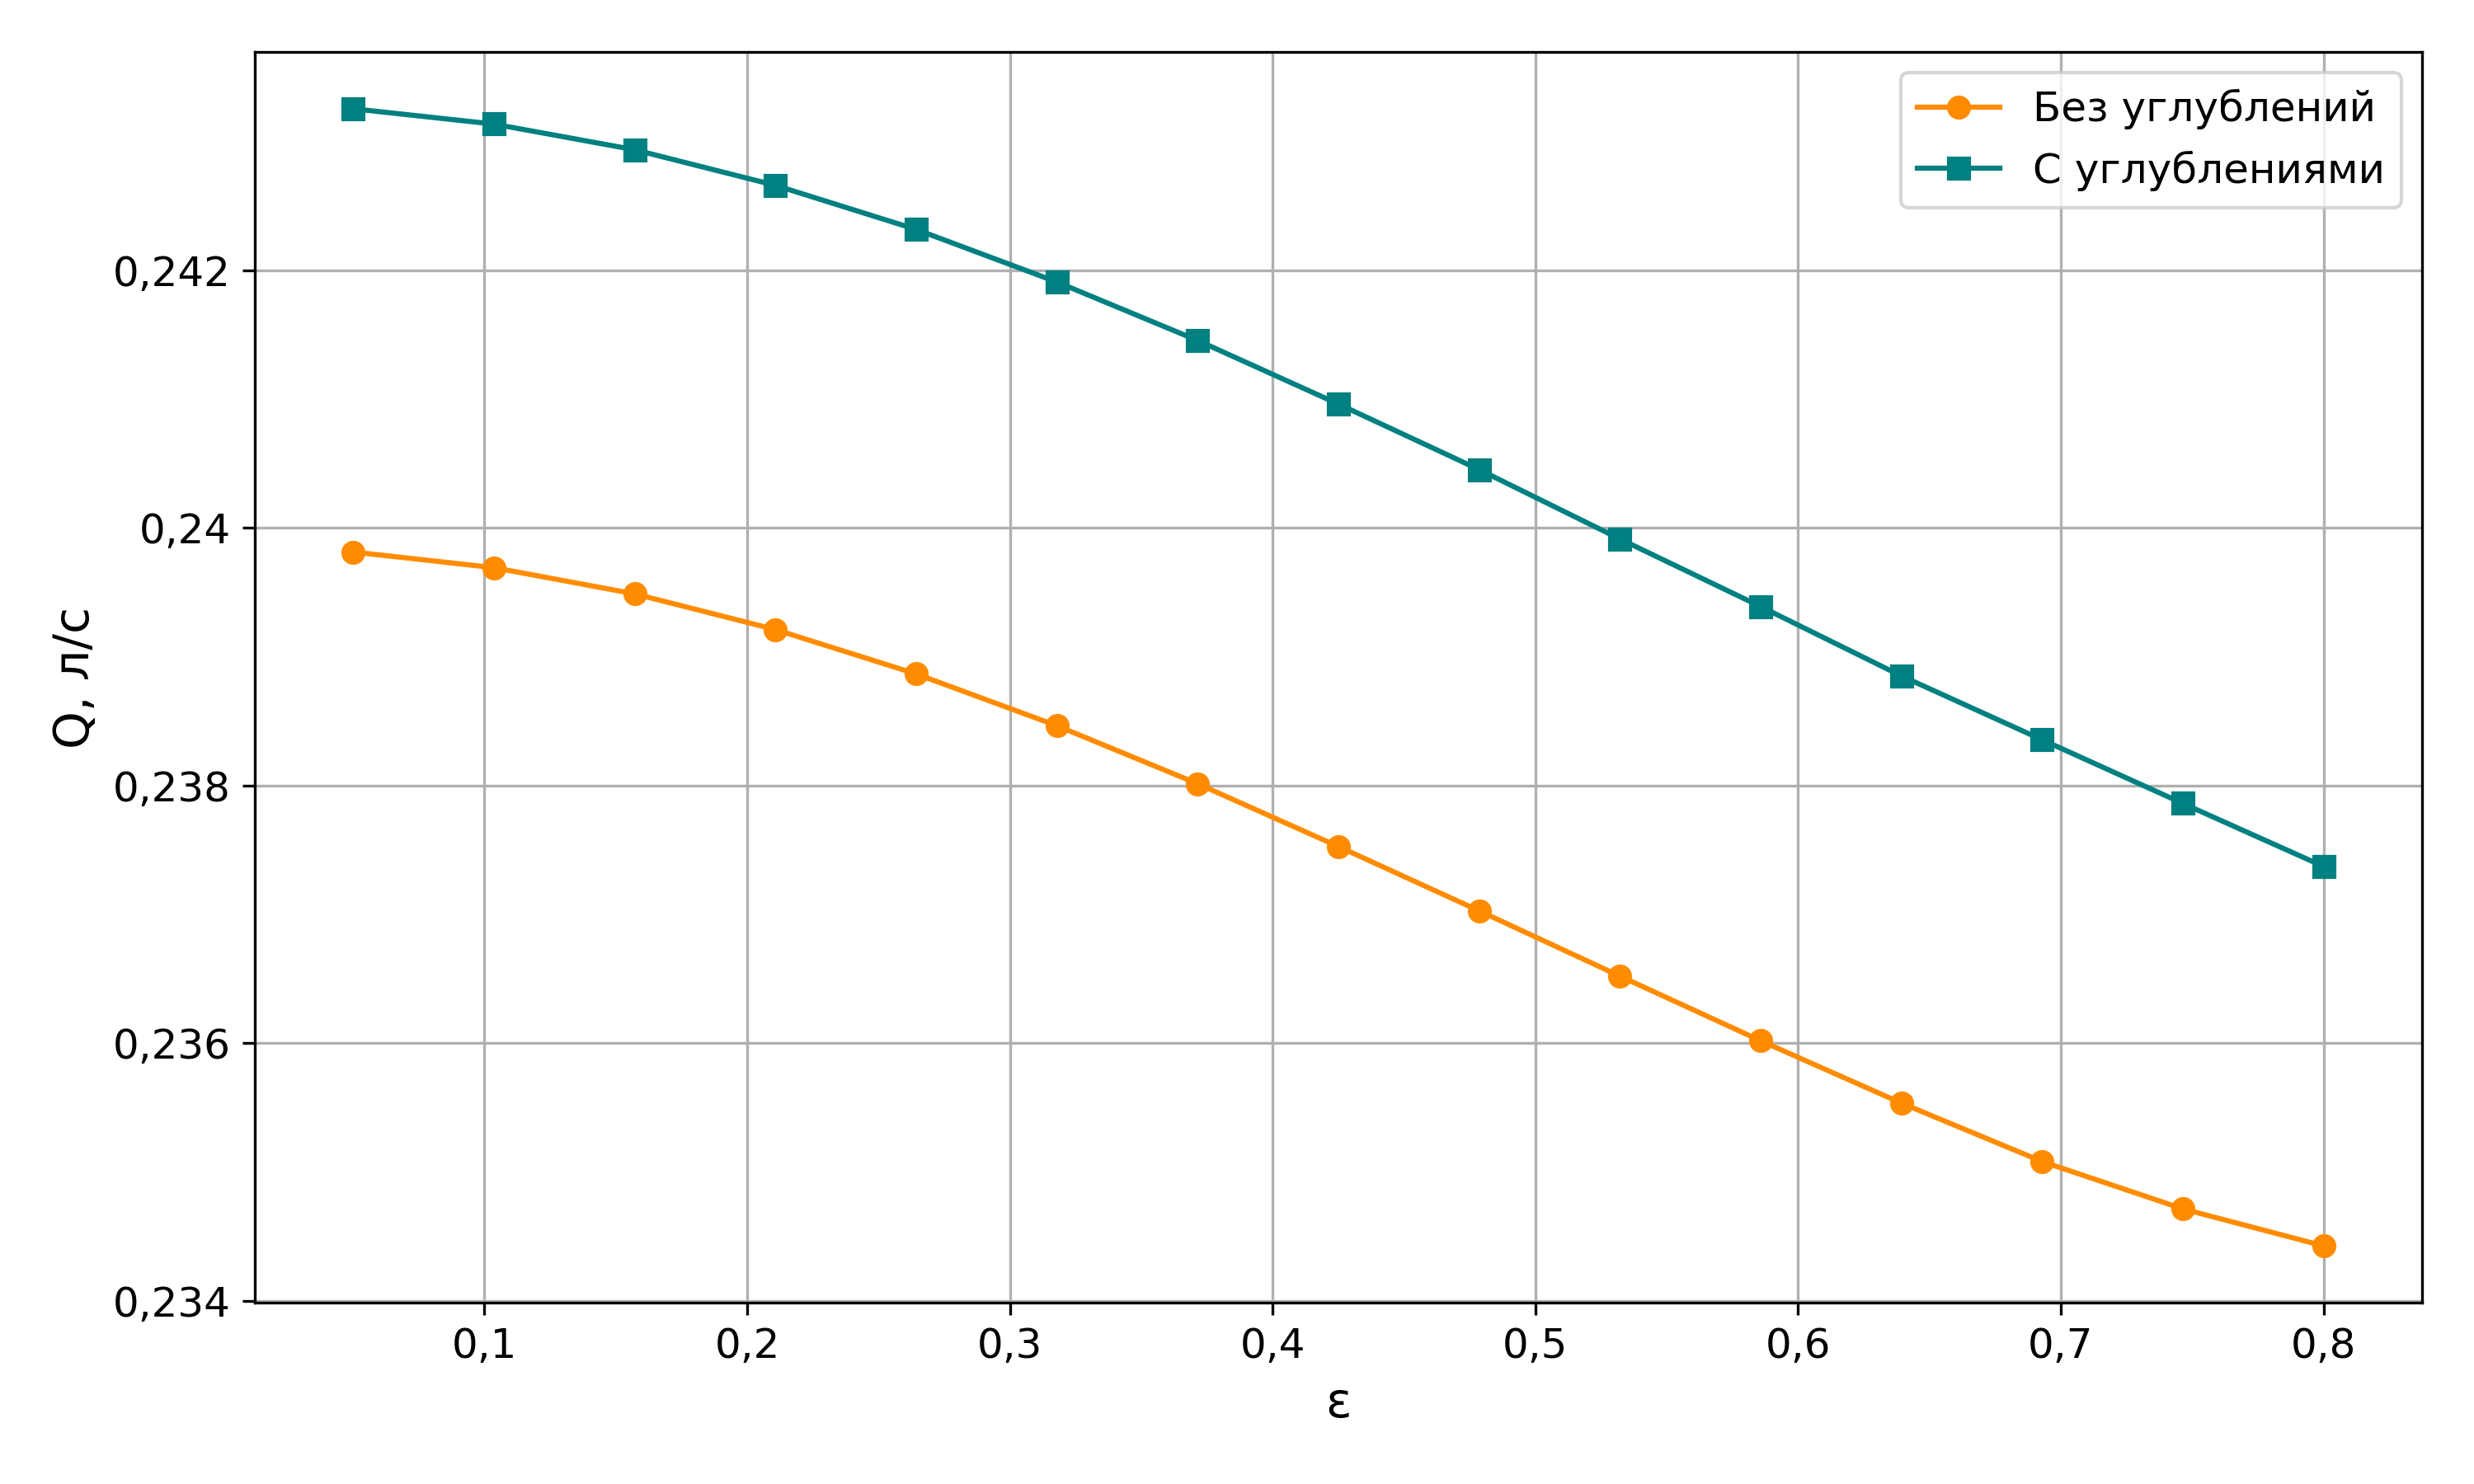
\includegraphics[width=\textwidth]{figures/flow_vs_epsilon.png}
\caption{Расход смазки $Q(\varepsilon)$ для гладкого и текстурированного подшипников}
\label{fig:flow_vs_eps}
\end{figure}

Расход смазки текстурированного подшипника незначительно превышает расход гладкого. Разница составляет порядка 1-1{,}5\% и практически не зависит от эксцентриситета.

Таким образом, текстурирование обеспечивает одновременное увеличение нагрузочной способности и снижение коэффициента трения при незначительном росте расхода. Эффект усиливается при увеличении эксцентриситета, что особенно важно для тяжелонагруженных подшипников.

\subsection*{Выводы по главе 3}
\phantomsection
\addcontentsline{toc}{subsection}{Выводы по главе 3}

Выполнен расчёт характеристик радиального подшипника скольжения с эллипсоидальным микрорельефом для 15 значений эксцентриситета. Получены поля давления и зазора, построены зависимости нагрузочной способности, коэффициента трения и расхода смазки от эксцентриситета. Сравнительный анализ при $\varepsilon = 0{,}6$ показал увеличение нагрузочной способности на $10{,}82$\%, снижение коэффициента трения на $11{,}78$\% и рост расхода на $1{,}43$\%, что подтверждает эффективность эллипсоидального текстурирования.
